\subsubsection{Magnetic lineations on the sea floor}
\label{sec:cookbooks-magnetic-stripes}
\textit{This section was contributed by Juliane Dannberg.}

The input file for this model can be found at \url{cookbooks/magnetic_stripes/magnetic_stripes.prm}.

This is a model of a mid-ocean ridge that shows how magnetic lineations 
are created on the sea floor as the magnetic field changes its orientation over time.
The model setup is similar to the heat flow model described in section~\ref{sec:cookbooks-heat-flow}. 
The only difference is that the model also has a compositional field that tracks the orientation of the
magnetic field when material reaches the surface at the ridge axis in the center of the model 
(and correspondingly, a value of 1 or -1 is assigned to the field). As the material is advected 
away from the ridge axis, alternating stripes -- symmetric with respect to the ridge axis -- become visible. 

This functionality is implemented through a new material model called magnetic stripes. 
This material model allows it to add a list of reversal times to the input file, that will then be used during the 
simulation. The input file used here contains the Earth's reversal history of the last 83 million years. 

Before the model can be run, the plugin needs to be compiled (see Section~\ref{sec:benchmark-run}). 
To illustrate the stripes forming on the sea floor, a high resolution is necessary, which means that this
cookbook needs longer to run than some of the others, and it may not always be feasible to run it on student laptops, 
or at least not during class. An animation can be found \href{https://www.youtube.com/watch?v=KeHNhWLL7ws}{here}.
Slides with an introduction to the Earth's magnetic field can be found \href{https://www.dropbox.com/s/2kkw3ce2muvn4nh/08_geophysics_lecture_02_05.pdf?dl=0}{here}.

\begin{figure}[h]
\phantom.
\hfill
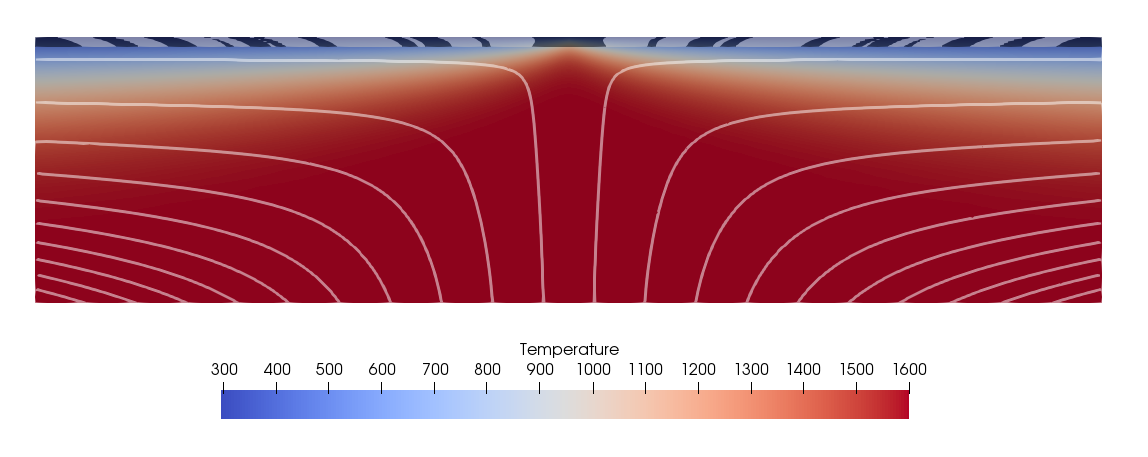
\includegraphics[width=0.6\textwidth]{mid-ocean-ridge.png}
\hfill
\phantom.
\caption{\it Setup of the mid-ocean ridge model. Background colors show temperature. Black and white colors at the top of the model illustrate the orientation of the magnetic field frozen in the rock when the melt generated at the mid-ocean ridge reaches the surface, crystallizes to form new sea floor, and the rock cools down. White lines illustrate the flow field.}
\label{fig:convection-box-iterations}
\end{figure}





